\documentclass{beamer}
\usetheme{CambridgeUS}

\usepackage{tikz}
\usepackage{xeCJK}
\usepackage{amsmath}
\usepackage[version=4]{mhchem}
\usetikzlibrary{graphs}
\usepackage{chemarr}
\usetikzlibrary{automata, positioning}
\usepackage{fontspec}
\usepackage{caption}
\usepackage{subfigure}
\usepackage{graphicx}


% 英文字体配置部分
\setmainfont{Source Serif Pro}%Times New Roman
\setsansfont{Source Sans Pro}
\setmonofont{Source Code Pro}
% 中文字体配置部分
\usepackage{xeCJK}%中文字体
\setCJKmainfont{宋体}%正文字体
\setCJKsansfont{黑体}%无衬线字体
\setCJKmonofont{楷体}%等宽字体
\setCJKfamilyfont{boldsong}{Source Han Serif SC Heavy}

\title[关于酶动力学的环流问题的研究]{硕士论文开题报告} 
\author{姜瑜浩}
\institute[CSRC]
{北京计算科学研究中心
\medskip
\textit{yuhaojiang@csrc.ac.cn}
} 
\begin{document}
    \frame{\titlepage}
	% \begin{frame}{课程成绩}
	% 	\begin{table}
	% 		\centering
	% 		\begin{tabular}{|c|c|c|c|c|c|}
	% 		\hline
	% 		课程名称	&学分&	成绩	&开课学校	& 任课教师&开课学期\\
	% 		\hline
	% 	  {偏微分方程数值解}& 3 & C & 北大 & 汤华中 & 秋季学期\\
	% 	  {凸优化}& 3 & C+ & 北大 & 文再文 & 秋季学期\\
	% 	  {偏微分方程(2)}&4 & B+ & 清华 & 简怀玉 & 秋季学期\\
	% 	  {基础泛函分析}& 4 & B & 清华 & 步尚全 & 秋季学期\\
	% 	  %{中国特色社会主义理论与实践}& 1 & 87 & 中物院 &\quad & 秋季学期\\
	% 	  %{中国马克思主义与当代}&	1 & 90 & 中物院 & \quad	& 秋季学期\\
	% 	  %{科学道德与学术诚信} & 1 & P & 中物院 & \quad & 秋季学期\\
	% 	  {有限元方法(2)}& 3 & A & 清华 & 郑春雄 & 春季学期\\
	% 	  {泛函分析(2)}& 4 & B- & 清华 & 步尚全 & 春季学期\\
	% 	  %{研究生综合英语}& 3 & 67 & 中物院 & 何英 & 春季学期\\
	% 	  %{自然辩证法与科技伦理}& 1 & 82 & 中物院 & \quad & 春季学期\\
	% 	  \hline
	% 	  \end{tabular}
	% 	  \end{table}
	% 	  总学分:26 学分 \; 公共课 \; 6学分 , 专业课和基础课 \; 20学分.
    % \end{frame}
    
	\begin{frame}{Enzymes: catalysts for biochemical reactions}
        Three-step Michaelis–Menten enzyme kinetics:
		$$
		E + S \xrightleftharpoons[k_{-1}]{k_1}
		ES \xrightleftharpoons[k_{-2}]{k_2}
		EP \xrightleftharpoons[k_{-3}]{k_3}
		E + P
		$$
		\begin{figure}[h]
			\centering
			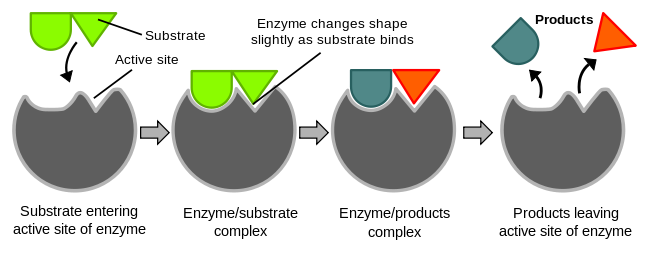
\includegraphics[scale=0.4]{enzyme.png}
	    \end{figure}
	\end{frame}

	\begin{frame}{Enzymes: catalysts for biochemical reactions}
		Three state Markov Chains:
		\begin{figure}[h]
			\centering
			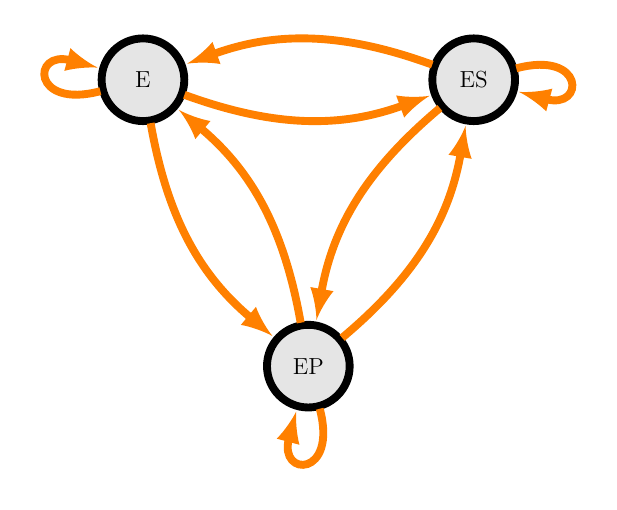
\begin{tikzpicture}[scale=0.7, font=\sffamily]
				\tikzstyle{every node} = [font=\large,scale=0.7]
				% Setup the style for the states
				\tikzset{node style/.style={state, 
											minimum width=1.5cm,
											line width=1mm,
											fill=gray!20!white}}
				% Draw the states
				\node[node style] at (0, 0)     (e)     {E};
				\node[node style] at (6, 0)     (es)     {ES};
				\node[node style] at (3, -5.196) (ep) {EP};
				% Connect the states with arrows
				\draw[every loop,
					  auto=right,
					  line width=1mm,
					  >=latex,
					  draw=orange,
					  fill=orange]
					(e)     edge[bend right=20]             (ep)
					(e)     edge[bend right=20, auto=left]  (es)
					(es)     edge[bend right=20]             (e)
					(es)     edge[bend right=20, auto=left]  (ep)
					(ep) edge[bend right=20]             (es)
					(ep) edge[bend right=20, auto=left]  (e)
					(e) edge[loop left] (e)
					(es) edge[loop right] (es)
					(ep) edge[loop below] (ep);
			\end{tikzpicture}
		\end{figure}
	\end{frame}

	\begin{frame}{Enzymes: catalysts for biochemical reactions}
		Cycle type in the three state Markov Chains:\\
		\begin{itemize}
			\item $E \longrightarrow E$
			\item $EP \longrightarrow EP$
			\item $ES \longrightarrow ES$
			\item $E \longrightarrow EP \longrightarrow E$
			\item $E \longrightarrow ES \longrightarrow ES$
			\item $ES \longrightarrow EP \longrightarrow ES$
			\item $E \longrightarrow EP \longrightarrow ES \longrightarrow E$
			\item $E \longrightarrow ES \longrightarrow EP \longrightarrow E$
		\end{itemize}
	\end{frame}

	\begin{frame}{Circulation of Recurrent Markov Chains}
		\begin{block}{Why study the cycles in the above Markov Chains?}
			For the above Markov Chains, if the cycle $E \rightarrow EP \rightarrow ES \rightarrow E$ occurs more frequently than $E \rightarrow ES \rightarrow EP \rightarrow E$, the whole chemical reaction is positive reaction, otherwise it is negative reaction.

		\end{block}
		\begin{block}{Can we use the cycle production process to represent the above Markov process?}
			Consider the Markov Chains $(\mathit{X}_i)_{i\in \mathbb{N}}$ until time $n>0$ , let $\mathit{X}_{i+1} = \mathit{X}_1$, then $\left(X_1, X_2, \dots, X_n, X_{n+1}\right)$ is a circuit, occuring along the sample path, it products a sequence of the sample cycles $\{\xi_1, \xi_2, \dots, \xi_j\}$, can we use this sequence to represent the Markov Chains uniquely?
		\end{block}
	\end{frame}

	\begin{frame}{Circulation of Recurrent Markov Chains}
		\begin{block}{Circulation Distribution}
			Let $X = (\mathit{X}_i)_{i\in \mathbb{N}}$ be a homogeneous, irreducible and
            positive recurrent Markov chain, with the transition matrix $\mathit{P}$, and the finite state space $\Gamma$.
            Let $\mathcal{C}_n$, $\mathit{w}_{c,n}$ represent the class of all cycles, and the number of times that the cycle $c$ has been formed until time $n>0$, respectively.
            % The sequence of sample weighted cycles $(\mathcal{C}_n, \mathit{w}_{c,n}/n)$ associated with the chain $X$ coverges almost surely to a class $(\mathcal{C}_{\infty}, \mathit{w}_{\infty})$, that is,
            As $n \rightarrow \infty$, we have:
			\begin{align*}
				\mathcal{C}_{\infty} &= \lim_{n \rightarrow +\infty} \mathcal{C}_n, \quad a.e. \\
                \mathit{w}_c &= \lim_{n \rightarrow +\infty} \frac{\mathit{w}_{c,n}}{n}, \quad a.e.\\
            % \end{align*}
            % and
            % \begin{align*}
                \mathit{w}_c &= \mathit{p}_{i_1, i_2} \mathit{p}_{i_2, i_3} \cdots \mathit{p}_{i_{s-1}, i_{s}} \mathit{p}_{i_s, i_1} \frac{\mathit{D}(\{i_1, i_2, \cdots i_s\}^c)}{\sum_{j\in \mathit{S}} \mathit{D}(\{j\}^c)}
            \end{align*}
            where $\mathit{D}(H)$ be the determinant of $I-P$ with rows and columns indexed in the index set $H$, and $\mathit{D}(\phi) = 1$
		\end{block}
	\end{frame}

	\begin{frame}{Large Deviations}
		\begin{block}{Laws of Large Number}
            The random variable $\left(\mathit{X}_i \right)$ takes their values in $\Gamma=\{1, \cdots, r\}$, and are i.i.d with marginal law $\rho=(\rho_s)_{s \in \Gamma}$. 
            We write
			$$ 
			\mathfrak{M}_1(\Gamma) = \{\nu = (\nu_1, \nu_2, \cdots, \nu_r)\in [0,1]^r:\sum_{s=1}^r \nu_s = 1\}
            $$ 
            to denote the probability simplex in $\mathbb{R}^r$, which may be identified with the set of probability measures on $\Gamma$.
            The values that occur along the sequence $\mathit{X}_1,..., \mathit{X}_n$ are recorded by means of the empirical measure $\mathit{L}_n = \frac{1}{n}\sum_{i=1}^{n}\delta_{\mathit{X}_i} $, and $\mathit{L}_n \in \mathfrak{M}_1(\Gamma)$, 
			According t o th e SLLN, we have
			\begin{figure}
				\centering
				\ce{$d(\mathit{L}_n, \rho)$ ->[$n\rightarrow \infty$] 0 $\quad$
				 $\mathbb{P} - a.s.$} 
			\end{figure}
			Above metric is the total variation distance:
			$$
			d(\mu, \nu) = \frac{1}{2} \sum_{s=1}^r |\mu_s - \nu_s|, \quad \mu, \nu \in \mathfrak{M}_1(\Gamma)
			$$
		\end{block}
	\end{frame}

	\begin{frame}{Large Deviations}
		\begin{block}{Level-1 Large Deviations (Cramers Theory)}
			Let $(\mathit{X}_i)$ 是上述定义的独立同分布的随机变量序列, 相应的经验测度为 $\mathit{L}_n = \frac{1}{n} \sum_{i=1}^n \delta_{\mathit{X}_i}$. 那么, 对于 $\forall a>0$, 
			$$
			\lim_{n \rightarrow \infty} \frac{1}{n} \log \mathbb{P} \left(\mathit{L}_n \in \mathit{B}_a^c(\rho)\right) = -\inf_{\nu \in \mathit{B}_a^c(\rho)} \mathit{I}(x)
			$$
			其中 $\mathit{B}_a(\rho)=\{\nu \in \mathfrak{M}_1(\Gamma): d(\nu,  \rho) \le a\}$ 是 $\rho$ 的邻域, $\mathit{B}_a^c(\rho) = \mathfrak{M}_1(\Gamma) \backslash  \mathit{B}_a(\rho)$, 且称
			$$
			\mathit{I}_{\rho}(\nu) = \sum_{s=1}^r \nu_s \log \left(\frac{\nu_s}{\rho_s}\right)
			$$
			为速率函数. 
		\end{block}
	\end{frame}

	\begin{frame}{大偏差理论}
		\begin{block}{Level-2 大偏差 (Sanov定理)}
			在随机变量序列 $(\mathit{X}_i)$ 上, 定义对经验测度
			$\mathit{L}_n^2 = \frac{1}{n} \sum_{i=1}^n \delta_{(\mathit{X}_i, \mathit{X}_{i+1})}$
			
			不妨令 $\mathit{X}_{n+1} = \mathit{X}_1$(当$n\rightarrow \infty$时, 该假设对$\mathit{L}_n^2$ 取值无影响. )
			则 $\mathit{L}_n^2$ 所在的概率测度空间
			$\widetilde{\mathfrak{M}}_1(\Gamma \times \Gamma) = \{\nu=(\nu_{st}) \in \mathfrak{M}_1(\Gamma \times \Gamma):$ \\$ \sum_{t} \nu_{st} = \sum_{t} \nu_{ts}, \forall s\}.$
		
			Sanov 证明了对于 $\forall a > 0$, 有:
			$$
			\lim_{n \rightarrow \infty} \frac{1}{n} \log \mathbb{P}(\mathit{L}_n^2 \in B_a^c(\rho \times \rho))
			= - \inf_{\nu \in B_a^c(\rho \times \rho)} \mathit{I}_{\rho}^2(\nu)
			$$
			其中 $B_a(\rho \times \rho) = \{\nu \in \widetilde{\mathfrak{M}}_1(\Gamma \times \Gamma): d(\nu, \rho \times \rho) \le a\}$, $\bar{\nu}_s = \sum_t \nu_{st}$, 且速率函数为
			$$
			\mathit{I}_{\rho}^2(\nu) = \sum_{s,t} \nu_{st} \log\left(\frac{\nu_{st}}{\bar{\nu_s}\rho_t}\right)
			$$
		\end{block} 
	\end{frame}

	\begin{frame}{环流的大偏差理论}
		\begin{block}{环流的大偏差理论}
			考虑上述环流问题的随机过程 $(\mathit{X}_i)_{i\in \mathbb{N}}$, 则 $C_{\infty}=\{c_1, c_2, \dots, c_s\}$ 为该过程所有可能环的集合, $\mathit{w} = \left(\mathit{w}_{c_1}, \mathit{w}_{c_2}, \dots, \mathit{w}_{c_s}\right)$ 为该马氏链的环流分布. 不妨令 $\mathit{X}_{n+1} = \mathit{X}_1$, 环流的经验测度为 $\mathit{w}_n = \left(\mathit{w}_{c_1, n}, \mathit{w}_{c_2, n}, \dots, \mathit{w}_{c_s, n}\right)$
			定义 $\mathit{w}_{c, n}$所在的空间:
			$$
			\mathfrak{M}_2 = \{\mu=\left(\mu_{c_1}, \mu_{c_2}, \dots, \mu_{c_s}\right)\in \left[0, 1\right]^s: \sum_{i=1} |c_i| \mu_{c_i}\}, 
			$$
			其中 $|c_i|$ 表示环 $c_i$ 中点的数量. 
			则对 $\forall a >0$, 有:
			$$
			\frac{1}{n} \log \mathbb{P} \left(\mathit{w}_n \in B_a^c(\mathit{w})\right) = - \inf_{\nu \in B_a^c(\mathit{w})} \mathit{I}^{c_1, c_2, \dots, c_s}(\nu)
			$$
		\end{block}
	\end{frame}

	\begin{frame}{速率函数及其性质}
		\begin{block}{Level-1 大偏差的速率函数}
			\begin{itemize}
				\item $\mathit{I}_{\rho}$ 是有界的, 连续的, 且在空间 $\mathfrak{M}_1(\Gamma)$是强凸的
				\item $\mathit{I}_{\rho} \ge 0$. 当且仅当 $\nu = \rho$ 时, 取等. 
				\item 通常称 $\mathit{H}(\nu | \rho) = \mathit{I}_{\rho}$ 为 $\nu$ 关于 $\rho$ 的交叉熵. 在信息论中, 通常用其表示两个函数分布之间的差别. 
			\end{itemize}
		\end{block}

		\begin{block}{Level-2 大偏差的速率函数}
			\begin{itemize}
				\item $\mathit{I}^2_{\rho}$ 是有界的, 连续的, 且在空间 $\widetilde{\mathfrak{M}}_1(\Gamma \times \Gamma)$ 是强凸的. 
				\item $\mathit{I}^2_{\rho}(\nu) \ge 0$. 当且仅当 $\nu = \rho \times \rho$ 时, 取等. 
				\item $\mathit{I}_{\rho}^2(\nu) = \mathit{H}(\nu | \bar{\nu} \times \rho)$为 $\nu$ 相对于 $\bar{\nu} \times \rho$ 的交叉熵. 
			\end{itemize}
		\end{block}
	\end{frame}

	\begin{frame}{速率函数及其性质}
		\begin{block}{环流大偏差的速率函数}
			$\mathit{I}^{c_1, c_2, \dots, c_s}$ 的存在性和下列性质, 已有文献给出了证明. 
			\begin{itemize}
				\item $\mathit{I}^{c_1, c_2, \dots, c_s}$ 是有界的, 连续的, 且在空间 $\mathfrak{M}_2$ 是凸的. 
				\item $\mathit{I}^{c_1, c_2, \dots, c_s}(\nu) \ge 0$. 当且仅当 $\nu = w$ 时, 取等. 
				\item 如果 $c_k$ 和 $c_l$ 相似(环包含的节点相同), 则有下式成立
				$$\mathit{I}^{c_1, c_2, \dots, c_s}(x_1, \dots, x_k, \dots, x_l, \dots, x_r) = \mathit{I}^{c_1, c_2, \dots, c_s}(x_1, \dots, x_l, \dots, x_k, \dots, x_r) - (\log \frac{\gamma^{c_k}}{\gamma^{c_l}} (x_k - x_l))$$
				\item 
			\end{itemize}
		\end{block}
		分析该酶促反应, 我们还需要知道该反应达到平稳状态的速率是多少?也就是环生成过程($\{\xi_{j}\}$)收敛到平稳分布($\mathit{w}$)的速率是多少?即 $\mathit{I}^{c_1, c_2, \dots, c_s}$ 的具体表达式是多少?

		
	\end{frame}

	\begin{frame}{速率函数及其性质}
		\begin{block}{净环流大偏差的速率函数}
			令 $c_l$ 表示环 $E \longrightarrow EP \longrightarrow ES \longrightarrow E$, $c_l^-$ 表示相应的反环 $E \longrightarrow ES \longrightarrow EP \longrightarrow E$, 称$\mathit{w}_{c_l} - \mathit{w}_{c_l^-}$为净环流. 
			对于上述酶促反应, 净环流达到平稳, 已经是一个动态平衡. 依据大偏差的收缩原理, 净环流的的大偏差是存在的, 则净环流的具体表达式是什么?
		\end{block}
	\end{frame}

	\begin{frame}{其他生化反应}
		上述环流大偏差的表达式能否推广到其他生化反应?
		\captionsetup[figure]{labelfont={bf},name={},labelsep=period}
		\begin{figure}[h]
			\begin{minipage}[t]{0.4\linewidth}
				\centering
				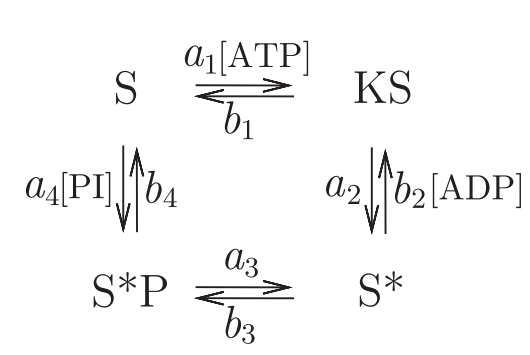
\includegraphics[scale=0.4]{phosphorylation_dephosphorylation_cycle.png}
				\caption{磷酸-脱磷酸化循环}
			\end{minipage}
			\begin{minipage}[t]{0.4\linewidth}
				\centering
				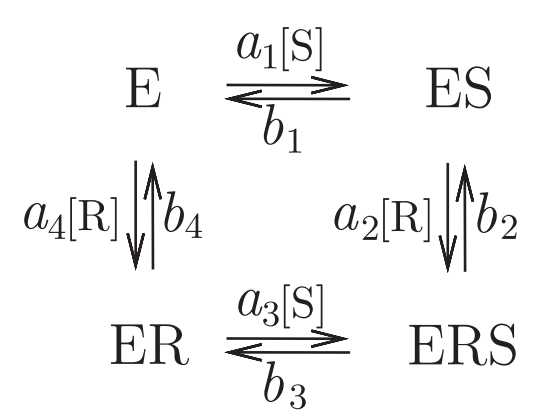
\includegraphics[scale=0.4]{general_modifier_machanism.png}
				\caption{广义的修正机制}
			\end{minipage}
			%\caption{四状态生化反应模型}
	    \end{figure}
		
		\begin{figure}[h]
			\begin{minipage}[t]{0.4\linewidth}
				\centering
				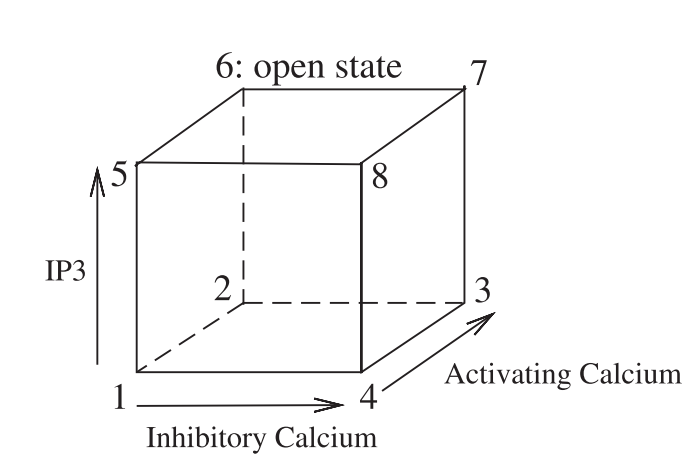
\includegraphics[scale=0.4]{De Young-Keizer model.png}
				\caption{De Young-Keizer 模型}
			\end{minipage}
			\begin{minipage}[t]{0.4\linewidth}
				\centering
				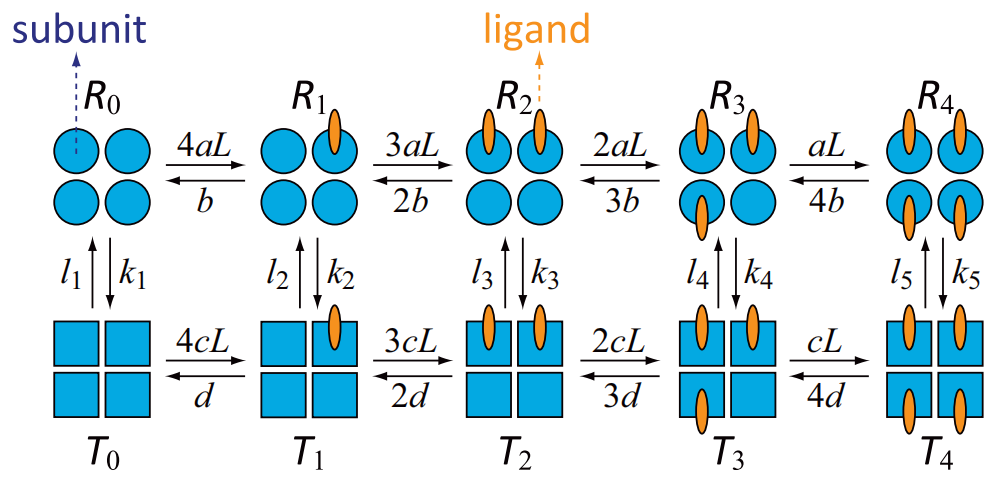
\includegraphics[scale=0.4]{MWC.png}
				\caption{MW模型}
			\end{minipage}
			%\caption{八状态生化反应模型}
	    \end{figure}
	\end{frame}
\end{document}